\documentclass{article}
\usepackage{tikz}
\usetikzlibrary{shapes.geometric, arrows}
\usetikzlibrary{shapes.misc, positioning}

\definecolor{lavander}{cmyk}{0,0.48,0,0}
\definecolor{violet}{cmyk}{0.79,0.88,0,0}
\definecolor{burntorange}{cmyk}{0,0.52,1,0}

\def\lav{lavander!90}
\def\oran{orange!30}

\tikzstyle{neighbors}=[draw,circle,violet,bottom color=\lav,
                  top color= white, font=\scriptsize,text=violet,minimum width=10pt]
\tikzstyle{queries}=[draw,circle,burntorange, left color=\oran,
                       text=violet,minimum width=30pt]

\tikzstyle{io} = [trapezium, trapezium left angle=70, trapezium right angle=110, minimum width=3cm, minimum height=1cm, text centered, draw=black, color=burntorange,left color=\oran,text=black]

\tikzstyle{res} = [trapezium, trapezium left angle=70, trapezium right angle=110, minimum width=3cm, minimum height=1cm, text centered, draw=black, color=violet,bottom color=\lav, top color=white,text=black]

\tikzstyle{process} = [rectangle, minimum width=3cm, minimum height=1cm, text centered, draw=violet, bottom color=\lav, top color=white]

\tikzstyle{grey} = [ rectangle, rounded corners=10pt, bottom color=black!10, top color=black!2] 

\tikzstyle{aro} = [->, thick,  shorten >=2pt, shorten <=2pt]

\begin{document}
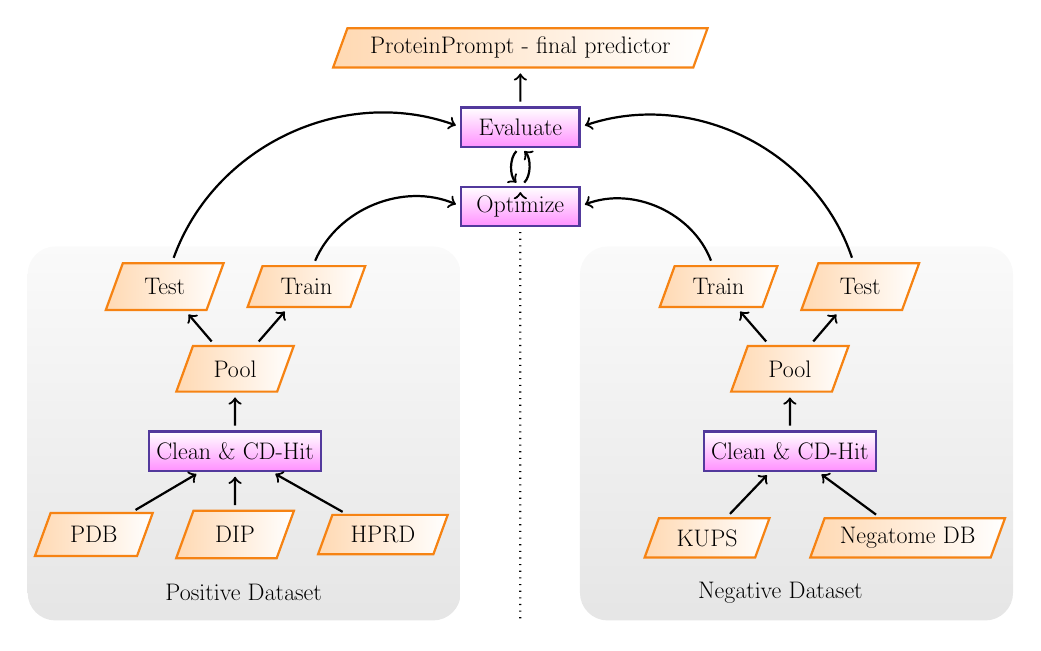
\begin{tikzpicture}[auto,thick, scale=0.5, transform shape,align=center, node distance = 1.5cm]

  \tikz {every node} = [font=\LARGE]
  
  \node (final) [io] { ProteinPrompt - final predictor};
  \node (apply) [process, below=1cm of final] {Evaluate}
  edge [aro] (final);
  \node (opt) [process,below=1cm of apply] {Optimize};

  \draw [aro,bend right=45] (apply.south) edge (opt.north)
                            (opt.north) edge (apply.south);


  \node[grey,minimum width=11cm,minimum height=9.5cm,below left=0.5cm and 0 of opt]{ \parbox[b][8.5cm]{4cm}{Positive Dataset}};
  
  \node (ptrain) [io,below left=1cm and 3.4cm of opt] {Train}
  edge[aro,bend left=45] (opt.west);

  \node (ptest)  [io,left=1cm of ptrain] {Test}
  edge[aro,bend left=45] (apply.west);

  \path (ptrain) -- node(ppool)[io,below=1.5cm]{Pool} (ptest);

  \draw [aro] (ppool) edge (ptest)
  edge( ptrain);

  \node (pclean) [process,below=1cm of ppool] {Clean \& CD-Hit}
  edge[aro](ppool);
  
  
  \node (ip1) [io, below=1cm of pclean] {DIP}
  edge[aro](pclean);
  \node (ip2) [io,right=1cm of ip1] {HPRD}
  edge[aro](pclean);
  \node (ip3) [io,left=1cm of ip1] {PDB}
  edge[aro](pclean);

  \node[grey,minimum width=11cm,minimum height=9.5cm,below right=0.5cm and 0 of opt]{ \parbox[b][8.5cm]{5cm}{Negative Dataset}};

  \node (ntrain) [io,below right=1cm and 3cm of opt] {Train}
  edge[aro,bend right=45] (opt.east);

  \node (ntest)  [io,right=1cm of ntrain] {Test}
  edge[aro,bend right=45] (apply.east);

  \path (ntrain) -- node(npool)[io,below=1.5cm]{Pool} (ntest);

  \node (nclean) [process,below=1cm of npool] {Clean \& CD-Hit}
  edge[aro] (npool);
  
  \draw [aro] (npool) edge (ntest)
  edge( ntrain);

  \node (ghost) [below=1.5cm of nclean]{};
  \node (in1) [io, right=0.5cm of ghost] {Negatome DB}
  edge[aro](nclean);
  \node (in2) [io, left=0.5cm of ghost] {KUPS}
  edge[aro](nclean);

  \draw [dotted, shorten <=2pt] (opt) edge (0,-14.6);
  
%  edge[aro, bend right=45] (ptest.north);

\end{tikzpicture}


\end{document}

  
